%\documentclass{standalone}
%\usepackage{tikz}
%\usetikzlibrary{patterns,plotmarks}
%\begin{document}
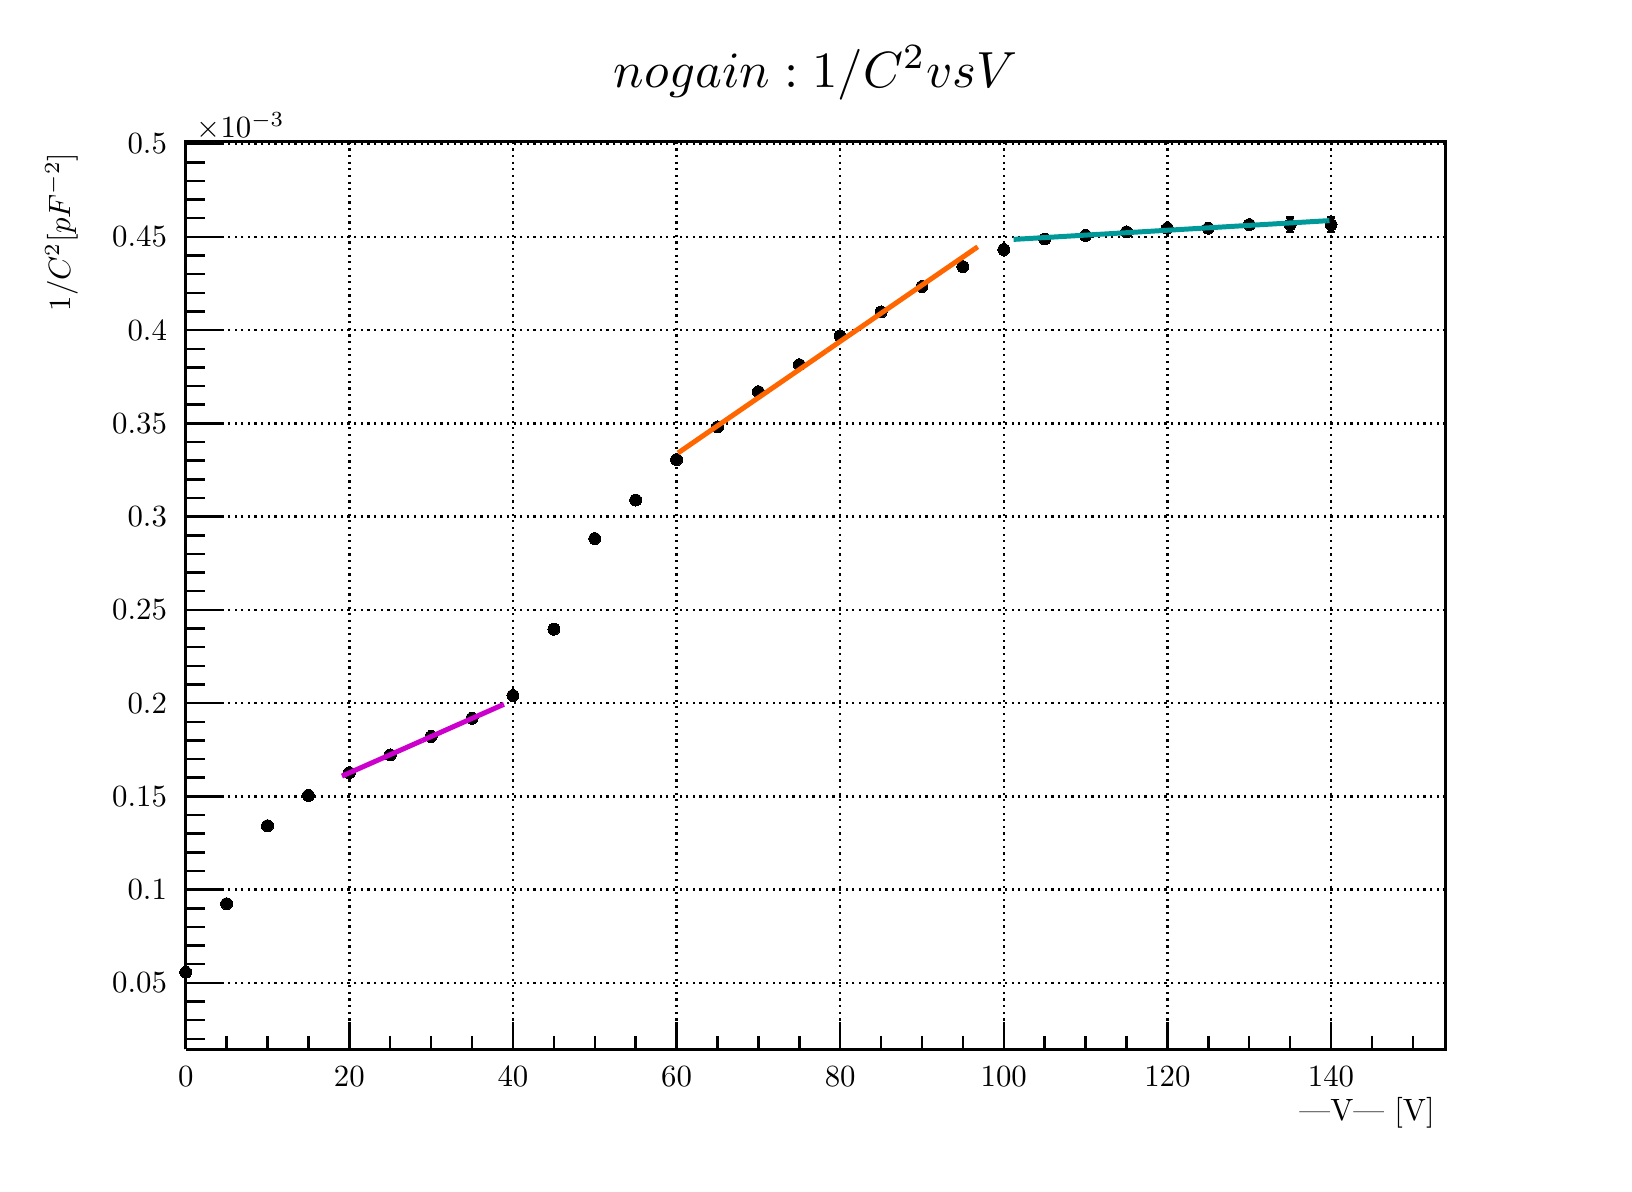
\begin{tikzpicture}
\def\CheckTikzLibraryLoaded#1{ \ifcsname tikz@library@#1@loaded\endcsname \else \PackageWarning{tikz}{usetikzlibrary{#1} is missing in the preamble.} \fi }
\CheckTikzLibraryLoaded{patterns}
\CheckTikzLibraryLoaded{plotmarks}
\pgfdeclareplotmark{cross} {
\pgfpathmoveto{\pgfpoint{-0.3\pgfplotmarksize}{\pgfplotmarksize}}
\pgfpathlineto{\pgfpoint{+0.3\pgfplotmarksize}{\pgfplotmarksize}}
\pgfpathlineto{\pgfpoint{+0.3\pgfplotmarksize}{0.3\pgfplotmarksize}}
\pgfpathlineto{\pgfpoint{+1\pgfplotmarksize}{0.3\pgfplotmarksize}}
\pgfpathlineto{\pgfpoint{+1\pgfplotmarksize}{-0.3\pgfplotmarksize}}
\pgfpathlineto{\pgfpoint{+0.3\pgfplotmarksize}{-0.3\pgfplotmarksize}}
\pgfpathlineto{\pgfpoint{+0.3\pgfplotmarksize}{-1.\pgfplotmarksize}}
\pgfpathlineto{\pgfpoint{-0.3\pgfplotmarksize}{-1.\pgfplotmarksize}}
\pgfpathlineto{\pgfpoint{-0.3\pgfplotmarksize}{-0.3\pgfplotmarksize}}
\pgfpathlineto{\pgfpoint{-1.\pgfplotmarksize}{-0.3\pgfplotmarksize}}
\pgfpathlineto{\pgfpoint{-1.\pgfplotmarksize}{0.3\pgfplotmarksize}}
\pgfpathlineto{\pgfpoint{-0.3\pgfplotmarksize}{0.3\pgfplotmarksize}}
\pgfpathclose
\pgfusepathqstroke
}
\pgfdeclareplotmark{cross*} {
\pgfpathmoveto{\pgfpoint{-0.3\pgfplotmarksize}{\pgfplotmarksize}}
\pgfpathlineto{\pgfpoint{+0.3\pgfplotmarksize}{\pgfplotmarksize}}
\pgfpathlineto{\pgfpoint{+0.3\pgfplotmarksize}{0.3\pgfplotmarksize}}
\pgfpathlineto{\pgfpoint{+1\pgfplotmarksize}{0.3\pgfplotmarksize}}
\pgfpathlineto{\pgfpoint{+1\pgfplotmarksize}{-0.3\pgfplotmarksize}}
\pgfpathlineto{\pgfpoint{+0.3\pgfplotmarksize}{-0.3\pgfplotmarksize}}
\pgfpathlineto{\pgfpoint{+0.3\pgfplotmarksize}{-1.\pgfplotmarksize}}
\pgfpathlineto{\pgfpoint{-0.3\pgfplotmarksize}{-1.\pgfplotmarksize}}
\pgfpathlineto{\pgfpoint{-0.3\pgfplotmarksize}{-0.3\pgfplotmarksize}}
\pgfpathlineto{\pgfpoint{-1.\pgfplotmarksize}{-0.3\pgfplotmarksize}}
\pgfpathlineto{\pgfpoint{-1.\pgfplotmarksize}{0.3\pgfplotmarksize}}
\pgfpathlineto{\pgfpoint{-0.3\pgfplotmarksize}{0.3\pgfplotmarksize}}
\pgfpathclose
\pgfusepathqfillstroke
}
\pgfdeclareplotmark{newstar} {
\pgfpathmoveto{\pgfqpoint{0pt}{\pgfplotmarksize}}
\pgfpathlineto{\pgfqpointpolar{44}{0.5\pgfplotmarksize}}
\pgfpathlineto{\pgfqpointpolar{18}{\pgfplotmarksize}}
\pgfpathlineto{\pgfqpointpolar{-20}{0.5\pgfplotmarksize}}
\pgfpathlineto{\pgfqpointpolar{-54}{\pgfplotmarksize}}
\pgfpathlineto{\pgfqpointpolar{-90}{0.5\pgfplotmarksize}}
\pgfpathlineto{\pgfqpointpolar{234}{\pgfplotmarksize}}
\pgfpathlineto{\pgfqpointpolar{198}{0.5\pgfplotmarksize}}
\pgfpathlineto{\pgfqpointpolar{162}{\pgfplotmarksize}}
\pgfpathlineto{\pgfqpointpolar{134}{0.5\pgfplotmarksize}}
\pgfpathclose
\pgfusepathqstroke
}
\pgfdeclareplotmark{newstar*} {
\pgfpathmoveto{\pgfqpoint{0pt}{\pgfplotmarksize}}
\pgfpathlineto{\pgfqpointpolar{44}{0.5\pgfplotmarksize}}
\pgfpathlineto{\pgfqpointpolar{18}{\pgfplotmarksize}}
\pgfpathlineto{\pgfqpointpolar{-20}{0.5\pgfplotmarksize}}
\pgfpathlineto{\pgfqpointpolar{-54}{\pgfplotmarksize}}
\pgfpathlineto{\pgfqpointpolar{-90}{0.5\pgfplotmarksize}}
\pgfpathlineto{\pgfqpointpolar{234}{\pgfplotmarksize}}
\pgfpathlineto{\pgfqpointpolar{198}{0.5\pgfplotmarksize}}
\pgfpathlineto{\pgfqpointpolar{162}{\pgfplotmarksize}}
\pgfpathlineto{\pgfqpointpolar{134}{0.5\pgfplotmarksize}}
\pgfpathclose
\pgfusepathqfillstroke
}
\definecolor{c}{rgb}{1,1,1};
\draw [color=c, fill=c] (0,0) rectangle (20,14.411);
\draw [color=c, fill=c] (2,1.4411) rectangle (18,12.9699);
\definecolor{c}{rgb}{0,0,0};
\draw [c,line width=0.9] (2,1.4411) -- (2,12.9699) -- (18,12.9699) -- (18,1.4411) -- (2,1.4411);
\definecolor{c}{rgb}{1,1,1};
\draw [color=c, fill=c] (2,1.4411) rectangle (18,12.9699);
\definecolor{c}{rgb}{0,0,0};
\draw [c,line width=0.9] (2,1.4411) -- (2,12.9699) -- (18,12.9699) -- (18,1.4411) -- (2,1.4411);
\draw [c,line width=0.9] (2,1.4411) -- (18,1.4411);
\draw [c,dash pattern=on 0.80pt off 1.60pt ,line width=0.9] (2,12.9699) -- (2,1.4411);
\draw [c,dash pattern=on 0.80pt off 1.60pt ,line width=0.9] (4.07792,12.9699) -- (4.07792,1.4411);
\draw [c,dash pattern=on 0.80pt off 1.60pt ,line width=0.9] (6.15584,12.9699) -- (6.15584,1.4411);
\draw [c,dash pattern=on 0.80pt off 1.60pt ,line width=0.9] (8.23377,12.9699) -- (8.23377,1.4411);
\draw [c,dash pattern=on 0.80pt off 1.60pt ,line width=0.9] (10.3117,12.9699) -- (10.3117,1.4411);
\draw [c,dash pattern=on 0.80pt off 1.60pt ,line width=0.9] (12.3896,12.9699) -- (12.3896,1.4411);
\draw [c,dash pattern=on 0.80pt off 1.60pt ,line width=0.9] (14.4675,12.9699) -- (14.4675,1.4411);
\draw [c,dash pattern=on 0.80pt off 1.60pt ,line width=0.9] (16.5455,12.9699) -- (16.5455,1.4411);
\draw [c,dash pattern=on 0.80pt off 1.60pt ,line width=0.9] (16.5455,12.9699) -- (16.5455,1.4411);
\draw [c,line width=0.9] (2,1.4411) -- (2,12.9699);
\draw [c,dash pattern=on 0.80pt off 1.60pt ,line width=0.9] (18,2.28671) -- (2,2.28671);
\draw [c,dash pattern=on 0.80pt off 1.60pt ,line width=0.9] (18,3.47101) -- (2,3.47101);
\draw [c,dash pattern=on 0.80pt off 1.60pt ,line width=0.9] (18,4.65531) -- (2,4.65531);
\draw [c,dash pattern=on 0.80pt off 1.60pt ,line width=0.9] (18,5.83962) -- (2,5.83962);
\draw [c,dash pattern=on 0.80pt off 1.60pt ,line width=0.9] (18,7.02392) -- (2,7.02392);
\draw [c,dash pattern=on 0.80pt off 1.60pt ,line width=0.9] (18,8.20822) -- (2,8.20822);
\draw [c,dash pattern=on 0.80pt off 1.60pt ,line width=0.9] (18,9.39252) -- (2,9.39252);
\draw [c,dash pattern=on 0.80pt off 1.60pt ,line width=0.9] (18,10.5768) -- (2,10.5768);
\draw [c,dash pattern=on 0.80pt off 1.60pt ,line width=0.9] (18,11.7611) -- (2,11.7611);
\draw [c,dash pattern=on 0.80pt off 1.60pt ,line width=0.9] (18,12.9454) -- (2,12.9454);
\draw [c,dash pattern=on 0.80pt off 1.60pt ,line width=0.9] (18,2.28671) -- (2,2.28671);
\draw [c,dash pattern=on 0.80pt off 1.60pt ,line width=0.9] (18,12.9454) -- (2,12.9454);
\draw [c,line width=0.9] (2,1.4411) -- (18,1.4411);
\draw [c,line width=0.9] (2,1.78697) -- (2,1.4411);
\draw [c,line width=0.9] (2.51948,1.61404) -- (2.51948,1.4411);
\draw [c,line width=0.9] (3.03896,1.61404) -- (3.03896,1.4411);
\draw [c,line width=0.9] (3.55844,1.61404) -- (3.55844,1.4411);
\draw [c,line width=0.9] (4.07792,1.78697) -- (4.07792,1.4411);
\draw [c,line width=0.9] (4.5974,1.61404) -- (4.5974,1.4411);
\draw [c,line width=0.9] (5.11688,1.61404) -- (5.11688,1.4411);
\draw [c,line width=0.9] (5.63636,1.61404) -- (5.63636,1.4411);
\draw [c,line width=0.9] (6.15584,1.78697) -- (6.15584,1.4411);
\draw [c,line width=0.9] (6.67532,1.61404) -- (6.67532,1.4411);
\draw [c,line width=0.9] (7.19481,1.61404) -- (7.19481,1.4411);
\draw [c,line width=0.9] (7.71429,1.61404) -- (7.71429,1.4411);
\draw [c,line width=0.9] (8.23377,1.78697) -- (8.23377,1.4411);
\draw [c,line width=0.9] (8.75325,1.61404) -- (8.75325,1.4411);
\draw [c,line width=0.9] (9.27273,1.61404) -- (9.27273,1.4411);
\draw [c,line width=0.9] (9.79221,1.61404) -- (9.79221,1.4411);
\draw [c,line width=0.9] (10.3117,1.78697) -- (10.3117,1.4411);
\draw [c,line width=0.9] (10.8312,1.61404) -- (10.8312,1.4411);
\draw [c,line width=0.9] (11.3506,1.61404) -- (11.3506,1.4411);
\draw [c,line width=0.9] (11.8701,1.61404) -- (11.8701,1.4411);
\draw [c,line width=0.9] (12.3896,1.78697) -- (12.3896,1.4411);
\draw [c,line width=0.9] (12.9091,1.61404) -- (12.9091,1.4411);
\draw [c,line width=0.9] (13.4286,1.61404) -- (13.4286,1.4411);
\draw [c,line width=0.9] (13.9481,1.61404) -- (13.9481,1.4411);
\draw [c,line width=0.9] (14.4675,1.78697) -- (14.4675,1.4411);
\draw [c,line width=0.9] (14.987,1.61404) -- (14.987,1.4411);
\draw [c,line width=0.9] (15.5065,1.61404) -- (15.5065,1.4411);
\draw [c,line width=0.9] (16.026,1.61404) -- (16.026,1.4411);
\draw [c,line width=0.9] (16.5455,1.78697) -- (16.5455,1.4411);
\draw [c,line width=0.9] (16.5455,1.78697) -- (16.5455,1.4411);
\draw [c,line width=0.9] (17.0649,1.61404) -- (17.0649,1.4411);
\draw [c,line width=0.9] (17.5844,1.61404) -- (17.5844,1.4411);
\draw [anchor=base] (2,0.965539) node[scale=1.11327, color=c, rotate=0]{0};
\draw [anchor=base] (4.07792,0.965539) node[scale=1.11327, color=c, rotate=0]{20};
\draw [anchor=base] (6.15584,0.965539) node[scale=1.11327, color=c, rotate=0]{40};
\draw [anchor=base] (8.23377,0.965539) node[scale=1.11327, color=c, rotate=0]{60};
\draw [anchor=base] (10.3117,0.965539) node[scale=1.11327, color=c, rotate=0]{80};
\draw [anchor=base] (12.3896,0.965539) node[scale=1.11327, color=c, rotate=0]{100};
\draw [anchor=base] (14.4675,0.965539) node[scale=1.11327, color=c, rotate=0]{120};
\draw [anchor=base] (16.5455,0.965539) node[scale=1.11327, color=c, rotate=0]{140};
\draw [anchor= east] (18,0.634085) node[scale=1.11327, color=c, rotate=0]{|V| [V]};
\draw [c,line width=0.9] (2,1.4411) -- (2,12.9699);
\draw [c,line width=0.9] (2.48,2.28671) -- (2,2.28671);
\draw [c,line width=0.9] (2.24,2.52357) -- (2,2.52357);
\draw [c,line width=0.9] (2.24,2.76043) -- (2,2.76043);
\draw [c,line width=0.9] (2.24,2.99729) -- (2,2.99729);
\draw [c,line width=0.9] (2.24,3.23415) -- (2,3.23415);
\draw [c,line width=0.9] (2.48,3.47101) -- (2,3.47101);
\draw [c,line width=0.9] (2.24,3.70787) -- (2,3.70787);
\draw [c,line width=0.9] (2.24,3.94473) -- (2,3.94473);
\draw [c,line width=0.9] (2.24,4.18159) -- (2,4.18159);
\draw [c,line width=0.9] (2.24,4.41845) -- (2,4.41845);
\draw [c,line width=0.9] (2.48,4.65531) -- (2,4.65531);
\draw [c,line width=0.9] (2.24,4.89217) -- (2,4.89217);
\draw [c,line width=0.9] (2.24,5.12903) -- (2,5.12903);
\draw [c,line width=0.9] (2.24,5.36589) -- (2,5.36589);
\draw [c,line width=0.9] (2.24,5.60276) -- (2,5.60276);
\draw [c,line width=0.9] (2.48,5.83962) -- (2,5.83962);
\draw [c,line width=0.9] (2.24,6.07648) -- (2,6.07648);
\draw [c,line width=0.9] (2.24,6.31334) -- (2,6.31334);
\draw [c,line width=0.9] (2.24,6.5502) -- (2,6.5502);
\draw [c,line width=0.9] (2.24,6.78706) -- (2,6.78706);
\draw [c,line width=0.9] (2.48,7.02392) -- (2,7.02392);
\draw [c,line width=0.9] (2.24,7.26078) -- (2,7.26078);
\draw [c,line width=0.9] (2.24,7.49764) -- (2,7.49764);
\draw [c,line width=0.9] (2.24,7.7345) -- (2,7.7345);
\draw [c,line width=0.9] (2.24,7.97136) -- (2,7.97136);
\draw [c,line width=0.9] (2.48,8.20822) -- (2,8.20822);
\draw [c,line width=0.9] (2.24,8.44508) -- (2,8.44508);
\draw [c,line width=0.9] (2.24,8.68194) -- (2,8.68194);
\draw [c,line width=0.9] (2.24,8.9188) -- (2,8.9188);
\draw [c,line width=0.9] (2.24,9.15566) -- (2,9.15566);
\draw [c,line width=0.9] (2.48,9.39252) -- (2,9.39252);
\draw [c,line width=0.9] (2.24,9.62938) -- (2,9.62938);
\draw [c,line width=0.9] (2.24,9.86624) -- (2,9.86624);
\draw [c,line width=0.9] (2.24,10.1031) -- (2,10.1031);
\draw [c,line width=0.9] (2.24,10.34) -- (2,10.34);
\draw [c,line width=0.9] (2.48,10.5768) -- (2,10.5768);
\draw [c,line width=0.9] (2.24,10.8137) -- (2,10.8137);
\draw [c,line width=0.9] (2.24,11.0505) -- (2,11.0505);
\draw [c,line width=0.9] (2.24,11.2874) -- (2,11.2874);
\draw [c,line width=0.9] (2.24,11.5243) -- (2,11.5243);
\draw [c,line width=0.9] (2.48,11.7611) -- (2,11.7611);
\draw [c,line width=0.9] (2.24,11.998) -- (2,11.998);
\draw [c,line width=0.9] (2.24,12.2348) -- (2,12.2348);
\draw [c,line width=0.9] (2.24,12.4717) -- (2,12.4717);
\draw [c,line width=0.9] (2.24,12.7086) -- (2,12.7086);
\draw [c,line width=0.9] (2.48,12.9454) -- (2,12.9454);
\draw [c,line width=0.9] (2.48,2.28671) -- (2,2.28671);
\draw [c,line width=0.9] (2.24,2.04985) -- (2,2.04985);
\draw [c,line width=0.9] (2.24,1.81299) -- (2,1.81299);
\draw [c,line width=0.9] (2.24,1.57613) -- (2,1.57613);
\draw [c,line width=0.9] (2.48,12.9454) -- (2,12.9454);
\draw [anchor= east] (1.9,2.28671) node[scale=1.11327, color=c, rotate=0]{0.05};
\draw [anchor= east] (1.9,3.47101) node[scale=1.11327, color=c, rotate=0]{0.1};
\draw [anchor= east] (1.9,4.65531) node[scale=1.11327, color=c, rotate=0]{0.15};
\draw [anchor= east] (1.9,5.83962) node[scale=1.11327, color=c, rotate=0]{0.2};
\draw [anchor= east] (1.9,7.02392) node[scale=1.11327, color=c, rotate=0]{0.25};
\draw [anchor= east] (1.9,8.20822) node[scale=1.11327, color=c, rotate=0]{0.3};
\draw [anchor= east] (1.9,9.39252) node[scale=1.11327, color=c, rotate=0]{0.35};
\draw [anchor= east] (1.9,10.5768) node[scale=1.11327, color=c, rotate=0]{0.4};
\draw [anchor= east] (1.9,11.7611) node[scale=1.11327, color=c, rotate=0]{0.45};
\draw [anchor= east] (1.9,12.9454) node[scale=1.11327, color=c, rotate=0]{0.5};
\draw [anchor=base west] (2,13.0204) node[scale=1.11327, color=c, rotate=0]{$\times10^{-3}$};
\draw [anchor= east] (0.422807,12.9699) node[scale=1.11327, color=c, rotate=90]{$1/C^{2} [pF^{-2}]$};
\foreach \P in {(2,2.42153), (2.51948,3.29232), (3.03896,4.28273), (3.55844,4.66838), (4.07792,4.95595), (4.5974,5.18168), (5.11688,5.41617), (5.63636,5.6462), (6.15584,5.93629), (6.67532,6.77821), (7.19481,7.92991), (7.71429,8.41831),
 (8.23377,8.9325), (8.75325,9.34688), (9.27273,9.79504), (9.79221,10.1379), (10.3117,10.5015), (10.8312,10.8084), (11.3506,11.1305), (11.8701,11.3828), (12.3896,11.6004), (12.9091,11.7342), (13.4286,11.7794), (13.9481,11.8249), (14.4675,11.8707),
 (14.987,11.8707), (15.5065,11.9168), (16.026,11.9168), (16.5455,11.9168)}{\draw[mark options={color=c,fill=c},mark size=2.162162pt, line width=0.000000pt, mark=*] plot coordinates {\P};}
\draw [c,line width=0.9] (16.026,11.9919) -- (16.026,12.0092);
\draw [c,line width=0.9] (16.026,11.8416) -- (16.026,11.8243);
\draw [c,line width=0.9] (15.9758,12.0092) -- (16.0761,12.0092);
\draw [c,line width=0.9] (15.9758,11.8243) -- (16.0761,11.8243);
\draw [c,line width=0.9] (16.5455,11.9919) -- (16.5455,12.0092);
\draw [c,line width=0.9] (16.5455,11.8416) -- (16.5455,11.8243);
\draw [c,line width=0.9] (16.4953,12.0092) -- (16.5956,12.0092);
\draw [c,line width=0.9] (16.4953,11.8243) -- (16.5956,11.8243);
\draw (10,13.8427) node[scale=1.83689, color=c, rotate=0]{$nogain: 1/C^{2} vs V$};
\definecolor{c}{rgb}{0.8,0,0.8};
\draw [c,line width=1.8] (3.98442,4.91297) -- (4.00519,4.92218) -- (4.02597,4.9314) -- (4.04675,4.94061) -- (4.06753,4.94983) -- (4.08831,4.95904) -- (4.10909,4.96826) -- (4.12987,4.97747) -- (4.15065,4.98669) -- (4.17143,4.9959) -- (4.19221,5.00512)
 -- (4.21299,5.01433) -- (4.23377,5.02354) -- (4.25455,5.03276) -- (4.27532,5.04197) -- (4.2961,5.05119) -- (4.31688,5.0604) -- (4.33766,5.06962) -- (4.35844,5.07883) -- (4.37922,5.08805) -- (4.4,5.09726) -- (4.42078,5.10648) -- (4.44156,5.11569) --
 (4.46234,5.12491) -- (4.48312,5.13412) -- (4.5039,5.14334) -- (4.52468,5.15255) -- (4.54545,5.16177) -- (4.56623,5.17098) -- (4.58701,5.18019) -- (4.60779,5.18941) -- (4.62857,5.19862) -- (4.64935,5.20784) -- (4.67013,5.21705) -- (4.69091,5.22627)
 -- (4.71169,5.23548) -- (4.73247,5.2447) -- (4.75325,5.25391) -- (4.77403,5.26313) -- (4.79481,5.27234) -- (4.81558,5.28156) -- (4.83636,5.29077) -- (4.85714,5.29999) -- (4.87792,5.3092) -- (4.8987,5.31841) -- (4.91948,5.32763) -- (4.94026,5.33684)
 -- (4.96104,5.34606) -- (4.98182,5.35527) -- (5.0026,5.36449);
\draw [c,line width=1.8] (5.0026,5.36449) -- (5.02338,5.3737) -- (5.04416,5.38292) -- (5.06494,5.39213) -- (5.08571,5.40135) -- (5.10649,5.41056) -- (5.12727,5.41978) -- (5.14805,5.42899) -- (5.16883,5.43821) -- (5.18961,5.44742) -- (5.21039,5.45663)
 -- (5.23117,5.46585) -- (5.25195,5.47506) -- (5.27273,5.48428) -- (5.29351,5.49349) -- (5.31429,5.50271) -- (5.33506,5.51192) -- (5.35584,5.52114) -- (5.37662,5.53035) -- (5.3974,5.53957) -- (5.41818,5.54878) -- (5.43896,5.558) -- (5.45974,5.56721)
 -- (5.48052,5.57643) -- (5.5013,5.58564) -- (5.52208,5.59485) -- (5.54286,5.60407) -- (5.56364,5.61328) -- (5.58442,5.6225) -- (5.6052,5.63171) -- (5.62597,5.64093) -- (5.64675,5.65014) -- (5.66753,5.65936) -- (5.68831,5.66857) -- (5.70909,5.67779)
 -- (5.72987,5.687) -- (5.75065,5.69622) -- (5.77143,5.70543) -- (5.79221,5.71465) -- (5.81299,5.72386) -- (5.83377,5.73308) -- (5.85455,5.74229) -- (5.87532,5.7515) -- (5.8961,5.76072) -- (5.91688,5.76993) -- (5.93766,5.77915) -- (5.95844,5.78836)
 -- (5.97922,5.79758) -- (6,5.80679) -- (6.02078,5.81601);
\draw [c,line width=1.8] (6.02078,5.81601) -- (6.04156,5.82522);
\definecolor{c}{rgb}{1,0.4,0};
\draw [c,line width=1.8] (8.25299,9.01696) -- (8.29143,9.0434) -- (8.32987,9.06984) -- (8.36831,9.09628) -- (8.40675,9.12272) -- (8.4452,9.14917) -- (8.48364,9.17561) -- (8.52208,9.20205) -- (8.56052,9.22849) -- (8.59896,9.25493) -- (8.6374,9.28137)
 -- (8.67584,9.30782) -- (8.71429,9.33426) -- (8.75273,9.3607) -- (8.79117,9.38714) -- (8.82961,9.41358) -- (8.86805,9.44003) -- (8.90649,9.46647) -- (8.94493,9.49291) -- (8.98338,9.51935) -- (9.02182,9.54579) -- (9.06026,9.57224) -- (9.0987,9.59868)
 -- (9.13714,9.62512) -- (9.17558,9.65156) -- (9.21403,9.678) -- (9.25247,9.70445) -- (9.29091,9.73089) -- (9.32935,9.75733) -- (9.36779,9.78377) -- (9.40623,9.81021) -- (9.44468,9.83666) -- (9.48312,9.8631) -- (9.52156,9.88954) -- (9.56,9.91598) --
 (9.59844,9.94242) -- (9.63688,9.96887) -- (9.67532,9.99531) -- (9.71377,10.0217) -- (9.75221,10.0482) -- (9.79065,10.0746) -- (9.82909,10.1011) -- (9.86753,10.1275) -- (9.90597,10.154) -- (9.94442,10.1804) -- (9.98286,10.2068) -- (10.0213,10.2333)
 -- (10.0597,10.2597) -- (10.0982,10.2862) -- (10.1366,10.3126);
\draw [c,line width=1.8] (10.1366,10.3126) -- (10.1751,10.3391) -- (10.2135,10.3655) -- (10.2519,10.3919) -- (10.2904,10.4184) -- (10.3288,10.4448) -- (10.3673,10.4713) -- (10.4057,10.4977) -- (10.4442,10.5241) -- (10.4826,10.5506) -- (10.521,10.577)
 -- (10.5595,10.6035) -- (10.5979,10.6299) -- (10.6364,10.6564) -- (10.6748,10.6828) -- (10.7132,10.7092) -- (10.7517,10.7357) -- (10.7901,10.7621) -- (10.8286,10.7886) -- (10.867,10.815) -- (10.9055,10.8415) -- (10.9439,10.8679) -- (10.9823,10.8943)
 -- (11.0208,10.9208) -- (11.0592,10.9472) -- (11.0977,10.9737) -- (11.1361,11.0001) -- (11.1745,11.0265) -- (11.213,11.053) -- (11.2514,11.0794) -- (11.2899,11.1059) -- (11.3283,11.1323) -- (11.3668,11.1588) -- (11.4052,11.1852) -- (11.4436,11.2116)
 -- (11.4821,11.2381) -- (11.5205,11.2645) -- (11.559,11.291) -- (11.5974,11.3174) -- (11.6358,11.3438) -- (11.6743,11.3703) -- (11.7127,11.3967) -- (11.7512,11.4232) -- (11.7896,11.4496) -- (11.8281,11.4761) -- (11.8665,11.5025) -- (11.9049,11.5289)
 -- (11.9434,11.5554) -- (11.9818,11.5818) -- (12.0203,11.6083);
\draw [c,line width=1.8] (12.0203,11.6083) -- (12.0587,11.6347);
\definecolor{c}{rgb}{0,0.6,0.6};
\draw [c,line width=1.8] (12.5138,11.7288) -- (12.5543,11.7312) -- (12.5948,11.7336) -- (12.6353,11.736) -- (12.6758,11.7384) -- (12.7164,11.7408) -- (12.7569,11.7432) -- (12.7974,11.7456) -- (12.8379,11.7481) -- (12.8784,11.7505) -- (12.919,11.7529)
 -- (12.9595,11.7553) -- (13,11.7577) -- (13.0405,11.7601) -- (13.081,11.7625) -- (13.1216,11.765) -- (13.1621,11.7674) -- (13.2026,11.7698) -- (13.2431,11.7722) -- (13.2836,11.7746) -- (13.3242,11.777) -- (13.3647,11.7794) -- (13.4052,11.7818) --
 (13.4457,11.7843) -- (13.4862,11.7867) -- (13.5268,11.7891) -- (13.5673,11.7915) -- (13.6078,11.7939) -- (13.6483,11.7963) -- (13.6888,11.7987) -- (13.7294,11.8011) -- (13.7699,11.8036) -- (13.8104,11.806) -- (13.8509,11.8084) -- (13.8914,11.8108)
 -- (13.9319,11.8132) -- (13.9725,11.8156) -- (14.013,11.818) -- (14.0535,11.8205) -- (14.094,11.8229) -- (14.1345,11.8253) -- (14.1751,11.8277) -- (14.2156,11.8301) -- (14.2561,11.8325) -- (14.2966,11.8349) -- (14.3371,11.8373) -- (14.3777,11.8398)
 -- (14.4182,11.8422) -- (14.4587,11.8446) -- (14.4992,11.847);
\draw [c,line width=1.8] (14.4992,11.847) -- (14.5397,11.8494) -- (14.5803,11.8518) -- (14.6208,11.8542) -- (14.6613,11.8567) -- (14.7018,11.8591) -- (14.7423,11.8615) -- (14.7829,11.8639) -- (14.8234,11.8663) -- (14.8639,11.8687) --
 (14.9044,11.8711) -- (14.9449,11.8735) -- (14.9855,11.876) -- (15.026,11.8784) -- (15.0665,11.8808) -- (15.107,11.8832) -- (15.1475,11.8856) -- (15.1881,11.888) -- (15.2286,11.8904) -- (15.2691,11.8929) -- (15.3096,11.8953) -- (15.3501,11.8977) --
 (15.3906,11.9001) -- (15.4312,11.9025) -- (15.4717,11.9049) -- (15.5122,11.9073) -- (15.5527,11.9097) -- (15.5932,11.9122) -- (15.6338,11.9146) -- (15.6743,11.917) -- (15.7148,11.9194) -- (15.7553,11.9218) -- (15.7958,11.9242) -- (15.8364,11.9266)
 -- (15.8769,11.9291) -- (15.9174,11.9315) -- (15.9579,11.9339) -- (15.9984,11.9363) -- (16.039,11.9387) -- (16.0795,11.9411) -- (16.12,11.9435) -- (16.1605,11.9459) -- (16.201,11.9484) -- (16.2416,11.9508) -- (16.2821,11.9532) -- (16.3226,11.9556)
 -- (16.3631,11.958) -- (16.4036,11.9604) -- (16.4442,11.9628) -- (16.4847,11.9652);
\draw [c,line width=1.8] (16.4847,11.9652) -- (16.5252,11.9677);
\end{tikzpicture}
%\end{document}
